%% FELthesis: LaTeX class for bachelor, master, and phd thesis in CTU FEL
%% template.tex: template file
%% (c) 2012 Vít Zýka, vit.zyka@seznam.cz
%%
%% 2012-12-17 v0.1 first version derived from cmpthesis.tex

\documentclass[msc,draft,czech]{felthesis} % or [...,czech] for thesis in Czech
%%\documentclass[msc,draft]{felthesis} % or [...,czech] for thesis in Czech
%%\documentclass[phd,draft]{felthesis} % or [...,czech] for thesis in Czech

%% --- your additional packages:
\usepackage[utf8]{inputenc}

%% --- usefull draft packages
%%\usepackage[notref]{showkeys} % show labels for referencies
%%\usepackage{showlabels}       % similar
%%\usepackage{showidx}          % show index entries on every page

%% ======================================================== thesis info
\startThesisInfo
  \Title{Dynamické vyvažování obtížnosti her pomocí metod teorie her}
  \Author{Lukáš Beran}
  \AuthorEmail{beranlukas@gmail.com} % optional
  %\ThesisUrl{http://fel.cvut.cz/???/???-bsc.pdf} % optional
  \Date{Květen 2013}
  \Department{Katedra kybernetiky}
  \Advisor{Branislav Bošanský}
  \KeywordsCz{Dynamické vyvažování obtížnosti her; adaptivní UI; teorie her; \dots}
  \KeywordsEn{Dynamic difficulty game balancing; adaptive AI; game theory; \dots}
  %\AssignmentPage{assignment.pdf} % insert official assignment if given
\stopThesisInfo

%% ============================== your definitions (abbreviations etc.)
%%\def\Ax{\mathbf{A}_{x}}

%% =========================================================== settings
\graphicspath{{fig/}{logo/}} % subdirectories where TeX finds pictures
%\bibliography{beranlu6mst.bbl}
\addbibresource{beranlu6mst.bib} % bibliography file


%% ========================================================== text body
\begin{document}

\MakeTitle

\startFrontMatter
  \startAcknowledgement
Text of acknowledgement\dots
\stopAcknowledgement

\endinput
%%
%% End of file `acknowledgement.tex'.

  \startDeclaration
\ifCzech
  Prohlašuji, že jsem předloženou práci vypracoval samostatně,
  a~že jsem uvedl veškeré použité informační zdroje v~souladu
  s~Metodickým pokynem o~dodržování etických principů při přípravě
  vysokoškolských závěrečných prací.
\fi
\ifEnglish
  I declare that I worked out the presented thesis independently
  and I quoted all used sources of information in accord with
  Methodical instructions about ethical principles for writing
  academic thesis.
\fi
\stopDeclaration

\endinput
%%
%% End of file `declaration.tex'.

  \startAbstractCz
  Text abstraktu česky\dots
\stopAbstractCz

\startAbstractEn
  Text of abstract in English\dots
\stopAbstractEn

\endinput
%%
%% End of file `abstract.tex'.

  \TableOfContents
	\listoffigures
  \startAbbreviations{%
  Preliminary text\dots
}
\abbrv[abbrv.]  explanation
\abbrv[...]     ...
\stopAbbreviations

\endinput
%%
%% End of file `abbreviations.tex'.

\stopFrontMatter

\startBodyMatter
  %\includeonly{ch01}
  \chapter{Úvod}
Some introductory text\dots

\section{Definice}

Dynamické vyvažování obtížnosti (dynamic difficulty adjustement, DDA) je obecným konceptem, jak přistupovat k návrhu programů, jež jsou využívány uživateli rozdílných schopností a zkušeností. 

Klasickým přístup je předdefinování několika rozdílných nastavení s odlišnými požadavky na dovednosti uživatelů, kteří si mezi těmito nastaveními volí ručně. Naopak dynamický, adaptivní přístup volbu nastavení nechává alespoň z části na samotném programu, který se rozhoduje na základě modelu uživatele.

Se zkratkou DDA se nejčastěji setkáme v oblasti počítačových her a simulací, ale toto prostředí není závaznou podmínkou. Příklady budou uvedeny v sekci \ref{sec:aplikacedda}. Cílem DDA je přizpůsobovat proměnné systému co nejlépe aktuálním potřebám uživatele.  S typem aplikace úsce souvisí druh potřeb uživatele. Lišit se budou potřeby pacientů využívajících rehabilitační programy a potřeby hráčů počítačových her. Dále se v textu zaměřím na využití DDA v počítačových hrách, případně v tzv. serious game, které mají za úkol udržet uživatele u užitečné činnosti formou zábavné hry.

Synonymy pro DDA jsou např. dynamic difficulty balancing, dynamic game balancing, auto-dynamic difficulty, adaptive difficulty. Ve čtyřech z pěti pojmů se vyskutuje slovo difficulty (obtížnost), které jsem doposud nezmínil. Vyvažování obtížnosti je základem velké většiny hry využívající koncept DDA. Myšlenka za tím je jednoduchá. Je-li hra pro hráče příliš snadná, hráč se nudí, hru opustí. Naopak je-li hra příliš obtížná, hráč je frustrován, hru opouští. V obou případech hra ztrácí své uživatele. U komerčních produktů se pak jedná o ztrátu financí. U programu využívaném při rehabilitaci se pak jedná o ztrátu motivace v pokračovaní rehabilitací. Obtížnost hry tedy přímo souvisí s její zábavností a udělat hru zábavnou pro co největší masu lidí je cílem DDA. Míra zábavnosti hry není závislá pouze na její obtížnosti. Jak lze definovat zábavu a jak ji lze měřit více popíši v kapitole \ref{sec:defzab}. 

Každé využití auto-dynamického vyvažování hry lze zařadit do několika kategorií z různých úhlů pohledu. Různé hry vyžadují různé přístupy a je dobré se zamyslet nad konkrétní hrou. Vybrat si z jakých kategorií by mělo být DDA použito. Designér hry by si měl položit několik následujících otázek :

\begin{enumerate}
	\item Měl by hráč vědět, jestli je DDA použito?
	\item Má být obtížnost měněna v průběhu hry, nebo pouze na začátku?
	\item Je hlavním cílem hry zábava, nebo něco jiného?
	\item Jakým způsobem může být ovlivňována obtížnost hry?
\end{enumerate}

Dle svých odpovědí každý určitě zvládne zařadit hru do následujících kategorií.

\subsection{Explicitní a implicitní}

První dělení rozlišuje stav, kdy je hráč obeznámen s dynamickou obtížností a kdy naopak je mu to zatajeno. Jestliže hráč dopředu ví, že se obtížnost hry mění dle jeho konání, jedná se o explicitní DDA. Pokud je snaha utajit dynamickou změnu obtížnosti, jedná se o implicitní DDA.

Explicitní použití by mělo být dobře známé i ze všedního života. Když mezi s sebou v něčem soutěží týmy, kteří nejsou svými schopnostmi vyrovnaní, často se přistoupí k nějakému handicapu pro ty silnější. Ať už se jedná o věnování náskoku při závodu v běhu mladšímu z bratrů, či o posazení zdravého člověka do kolečkového křesla na paralympiádě. 

Příkladem ze světa deskových her může být ve hře Go povolení slabšímu hráči na začátku hry zahrát několik svých kamenů navíc, nebo naopak odebrání některých figur ve hře šachy hráči silnějšímu.

Někdy zařazení hry nemusí být zcela jednoznačné. Mnoho hráčů z laické veřejnosti je si vědomo podvádění v závodních hrách jako je Mario Kart, či Need For Speed, přestože se o tom nedozvědí v pravidlech hry. V případě, že se vývojáři rozhodnou pro implicitní DDA, měli by jej navrhnout tak, aby jej hráč neodhalil. Jestliže o něm každý ví, asi už není zcela korektní hru zařadit do implicitní kategorie.

\begin{figure}
  \centering
  
\includegraphics[width=0.5\textwidth]{ch1mariokart2}
	\caption{Ukázka špatného vyvažování hry u hry Mario Kart dává prostor pro vytváření vtipů. \cite{15UnTrue} }
	\label{ch1mariokart2}
\end{figure}

Nejasná kategorizace může být i v opačném případě. Mějme jako příklad moderní deskovou hru Vysoké napětí. Ve hře existují pravidla závislá na aktuálním pořadí hráčů a snaží se pomáhat prohrávajícím hráčům a naopak ubližovat těm ve vedení. U Vysokého napětí hráči nakupují suroviny v opačném pořadí než si vedou. Stejné suroviny mají rozdílnou cenu. Poslední hráč vykoupí nejlevnější suroviny a naopak na toho prvního zůstanou ty nejdražší. Za stejnou věc zaplatí různě, a tedy se zvýší šance posledního hráče dostat se do vedení. Přestože toto pravidlo je všem zúčastněným známo, tak asi málokdo o něm přemýšlí jako o dynamické vyvažování obtížnosti hry.

\subsection{Dynamická a statická}

Obtížnost hry lze přizpůsobovat před začátkem hry nebo v jejím průběhu. Dle toho se rozděluje DDA na statickou(offline), či dynamickou(online). Typický příkladem offline adaptivity bude zpracování hráčových dat a úprava hry během jejího načítání. Z tohoto důvodu je offline adaptivita zaměřena především na generování herního světa, herních scénářů a úkolů\cite{16Survey}. Příkladem mohou být hry Fallout 3 a Fallout: New Vegas, kde se při vstupu na nové území generují nepřátelé, a to dle levelu hráčova avatara. Offline adaptivitu lze považovat za jedinou možnou při vytváření různých logických hádanek a her. Na základě rychlosti řešení/nedokončení předchozí hádanky, lze vygenerovat hádanku novou lépe odpovídající hráčovým schopnostem. Tímto problémem se zabývá článek Automatic Generation of Game Elements via Evolution\cite{17Evol}, kde testovanými hrami byla hra se šachovými figurami a hra procházení barevným bludištěm.

Online adaptivita bude naopak zaměřena na adaptivitu umělé inteligence NPC a úpravu pravidel hry. Vede-li si hráč příliš dobře v závodní hře, ostatním hráčů se zvýší maximální rychlost. Ztratí-li hráč příliš životů, v rohu v další místnosti se objeví lékárnička. Adaptivita může být samozřejmě i druhým směrem. Sebere-li hráč soupeři důležité figurky v deskové hře šachy, soupeři se zvýší "inteligence", začne uvažovat na více kol dopředu. 

Online adaptivitu můžeme zasadit přímo do principů hry. Ve hře Pocket Billiards hrají proti sobě dva hráči na kulečníkovém stole. Na stole je několik koulí dvou barev. Každý hráč má přiřazenou jednu z barev a jeho úkolem je dostrkat své koule do děr dříve než to udělá soupeř. Adaptivita je zde dána samotným principem hry. Dostane-li se jeden hráč do vedení a odstraní z plochy znatelně více koulí než jeho soupeř, pak je pro něj stále obtížnější dostat další koule do děr. Zároveň se zvyšuje pravděpodobnost, že bude muset provést takový šťouch, který může odstranit z plochy soupeřovu koule, a tedy mu tím může pomoci dorovnat skóre.\cite{5}

\section{Aplikace DDA} \label{sec:aplikacedda}

Algoritmy vyvažování obtížnosti lze využít v širokém spektru aplikací. Mohou být vhodné všude tam, kde je vyžadována určitá dovednost, schopnost. V takovém případě může být obtížné aplikaci, program navrhnout tak, aby byl dobře využitelný velkým spektrem lidí různých schopností.

DDA můžeme nalézt nejen v zábavním průmyslu, ale i u vážných her. Adaptivní obtížnost programu může zefektivňovat léčbu nemocných lidí, nahrazovat osobního trenéra či učitele. V následujících 4 podkapitolách popisuji konkrétní užití dynamické obtížnosti v komerční i v akademické sféře.

\subsection{Zábavní průmysl}

Hráče počítačových her lze rozdělit dle jejich schopností od příležitostných až po hardcore hráče. Většina her obsahuje statickou volbu obtížnosti na začátku hry. V některých případech to nemusí být dostačující, a proto se tvůrci komerčních her snaží více, či méně úspěšně implementovat adaptivní obtížnost.

Na stránce \cite{1} lze nalézt desítky příkladů všech různých žánrů. Do následujícího seznamu 5 her jsem vybral ty známější příklady.


\subsubsection{Left 4 Dead}
\label{sec:Left4Dead}

V zombie hře Left 4 Dead pojmenovali adaptivní systém The AI Director. Na základě aktuálního hráčova zdraví, munice a relativní pozice v rámci dané úrovně hry The AI Director generuje ve hře zbraně, munici, lékárničky na pomoc hráči a naopak generuje lehčí, či těžší nepřátele. Např. blíží-li se hráč konci úrovně a má plné zdraví i munici, hra vygeneruje těžkého soupeře „Tank“. \cite{2}

\subsubsection{Max Payne 3}

Hra Max Payne 3 obsahuje celkem 5 statických obtížností(Easy, Medium, Hard, Hardcore, Old School), které se v průběhu hry adaptivně přizpůsobují hráči. Čím nižší obtížnost si hráč na začátku zvolí, tím více se hra může měnit ve prospěch hráče.

Jestliže hráč opakovaně umírá, dostane se mu pomoci ve formě bonusových léků(painkillers), které umožní lehčí projití daného úseku hry. Při smrti na lehkou a střední obtížnost se hráčův avatar obnoví minimálně s jedním plným zásobníkem pro každou zbraň vyjma granátometů. Plus za každé tři úmrtí ve stejném úseku dostane jeden painkiller navíc až do maximálního limitu devíti painkillerů.
Na těžkou obtížnost je dynamická obtížnost více limitovaná. Jestliže hráč zemře 5 krát po sobě, dostane jeden painkiller. Pokud zemře podesáté, dostane druhý painkiller. Další léky mu hra již nepřidává. \cite{3}

\subsubsection{The Elder Scrolls IV: Oblivion}

Dalším příkladem mohou být hry Oblivion a Fallout 3 od Bethesda Softworks. V Oblivionu nepřátelé levelují s hráčem. Stráže ve městě mají level o 2-5 vyšší než vy, banditi mají level o 2-5 nižší atd. Tímto je docíleno, že se můžete vydat kamkoli ve hře aniž byste narazili na příliš obtížné nepřátele. Mimo síly nepřátel se adaptivně upravuje druh nepřátel, jejich vybavení, nabízení zboží v obchodech apod. Občas může docházet k nelogickým situacím, kdy obyčejní potulní bandité mají na sobě nejmodernější brnění, nebo kdy máte za úkol donést vlčí kožešinu ve světe, kde už tak slabí nepřátelé se nepohybují. \cite{4}

\subsubsection{Mario Kart Wii}

Závodní simulátory jsou dobře známé využíváním adaptivní obtížnosti her a mezi nejznámější zástupce patří arkádové závody Mario Kart. Ve hře se adaptivně mění rychlost protivníků a také bonusové power-upy, které můžete sbírat. Hra podporuje natolik prohrávající hráče, že ať už je aktuální stav hry jakýkoli, může vyhrát kdokoliv.

Což lze brát jako velkou výhodu, kdy žádný z hráčů nemá důvod ke vzdávání hry. Nevýhodou je právě známost a odhalení tohoto systému, a tudíž je lehce zneužitelná. Např. konkrétně ve variantě Mario Kart Wii je vedoucí hráč na začátku posledního kola bombardován modrým krunýřem, či jinou devastující zbraní a je záhy poslán na poslední místo. Nejlepší strategií je projet do posledního kola na druhé pozici, což moc nedává smysl. \cite{5}

\subsubsection{Pro Evolution Soccer 2008}

Úspěšný fotbalový simulátor Pro Evolution Soccer se ve své verzi s číslem 2008 chlubil adaptivním systémem nazvaný Teamvision. Teamvision se učí od hráče jeho styl hry a snaží se upravovat taktiku svého týmu, aby co nejlépe reagovala na tu soupeřovu. Použití jedné finty může fungovat jednou, dvakrát, ale později již naprosto stejná finta nevede k vítězství. \cite{6}

\subsection{Cvičení}

Herní zařízení jako jsou Microsoft Kinect a Nintendo Wii dávají prostor pohybovým hrám. Stejně jako v jiných příkladech i zde platí, že existují lidé s diametrálně odlišnou fyzickou kondicí. Kondice se v ideálním případě při opakované hře stále zlepšuje, a proto je vhodné k tomu přizpůsobovat obtížnost hry.

Příkladem takové aplikace může být jednoduchá chodící hra hratelná v internetovém prohlížeči, jež má za úkol motivovat starší lidi k pohybu.

V druhém případě nebylo využito žádné ze zmíněných zařízení. Autoři článku \cite{7} se zaměřili na jogging v páru. 

\subsubsection{Podpora pohybu starších lidí}

Evropská populace stárne a odmítání pohybu staršími lidmi se stává závažným problémem. Z nedostatku fyzické námahy klesá síla a ohebnost těchto lidí, ztrácejí kostní hmotu a tím zvyšují pravděpodobnost pádu a zlomení některé z končetin. Z tohoto důvodu se skupina z Technologického institutu zaměřila na vývoj hry, jež má starší lidi motivovat k pohybu a jejíž nedílnou součástí je vyvažování obtížnosti. \cite{8}

Hra je vytvářena v HTML5 pro běžné použití ve webových prohlížečích a využívá Microsoft Kinect ovládání.

Základním cílem hry je udělat předem dané množství kroků v každé hře. Kroky jsou zaznamenávány pomocí Kinectu. Hráč musí jít v rytmu a zároveň se musí vyhýbat dírám v zemi. V případě špatných, či propásnutých kroků hráčův avatar zpomalí.

Při hře více hráčů se všichni zúčastnění snaží jít ve stejném tempu. Obtížnost je upravována přidáváním, či odebíráním překážek pro jednotlivé hráče a tím je motivuje k opakovanému hraní.

\begin{figure}
  \centering
  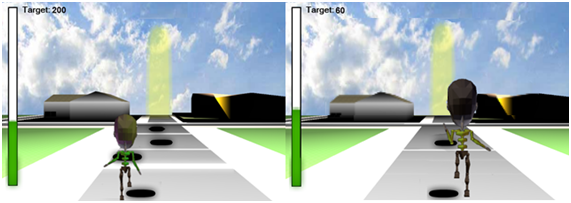
\includegraphics{ch1elderlypeople}
	\caption{Screenshoty HTML5 hry. Vlevo hraje nadaný hráč, vpravo s menší dovedností. \cite{8} }
	\label{ch1elderlypeople}
\end{figure}

\subsubsection{Jogging na dálku}

Ne každého baví běhat po parku samostatně a zároveň může být těžké najít někoho, kdo by si s vámi zaběhal ve stejnou dobu. Řešením může být jogging na dálku (jogging over distance), kdy dva lidé běží ve stejnou dobu, ale každý běží jinde, třeba i v jiném státě. Oba cvičící se dorozumívají přes telefon se sluchátky na hlavě. Povídají si, navzájem se podporují.

Různí lidé mají různou fyzickou kondici a může být problém se navzájem přizpůsobit v běhu tak, aby oba dva jedinci byli přibližně stejně namáhání. Neměla by nastat situace, kdy jeden udýchaně nemůže skoro mluvit a druhému naopak cvičení nic nedává.

V článku Balancing Exertion Experiences \cite{7} popisují svůj přístup k dané problematice. Každý z joggujících partnerů má při sobě chytrý telefon a měřič srdeční frekvence. Na telefonu mají nastavenou svojí ideální, cílovou srdeční frekvenci každý dle své fyzické kondice, případně dle doporučení doktora. Jestliže oba partneři mají srdeční frekvenci relativně stejnou vůči své cílové, pak je vše v pořádku. Partneři mohou běžet několik minut s cílovou srdeční frekvencí, poté se vyhecují, že na chvíli zrychlí a běží např. na 120\% své cílové frekvence. Pokud nastane situace, kdy první partner běží na 80\%, druhý na 110\%, jak vhodně donutit prvního zrychlit a druhého zpomalit? 

Autoři článku přišli se zajímavým řešením. Pomocí sluchátek mohou simulovat vjem, kdy se partneři slyší vedle sebe, kdy jeden slyší druhého před sebou, případně za sebou. Ve výše uvedeném příkladu by partner běžící na 110\% slyšel spoluběžce za ním, což by ho donutilo zpomalit. Opačně partner běžící na 80\% by slyšel toho druhého před sebou a byl by donucen zrychlit, aby se ve výsledku slyšeli co nejlépe, vedle sebe.

\subsection{Zdravotnictví}

Aplikace s adaptivní obtížností mohou pomáhat i nemocným lidem. Lidé po vážných úrazech se mnohdy učí, jak se vrátit zpět do normálního života. Při rehabilitaci lze mnohdy využít i počítačových her, které více motivují ke cvičení. Jestliže je taková hra příliš obtížná, pacient o ní brzy ztratí zájem. To platí i v opačném případě, kdy hra nutí pacienta provádět věci, které již bez problémů zvládá. Z těchto důvodů je velice vhodné obtížnost adaptivně měnit vůči konkrétním pacientům. Příkladem této aplikace je následující podkapitola Rehabilitace po utrpění mozkové mrtvice.

Druhá podkapitola v této sekci popisuje program asistující lidem trpícím demencí při jednoduchých úkolech.

\subsubsection{Rehabilitace po utrpění mozkové mrtvice}

Po cévní mozkové příhodě může dojít k částečnému až k v úplnému ochrnutí některých končetin. Pomocí různých cvičení lze tento dopad zvrátit. Mimo jiné mohou dobře posloužit jednoduché počítačové hry ovládané haptickým zařízením s adaptivním odporem a senzory. Obtížnost hry spočívá především v odporu ovladače a vzdálenosti, kterou musí osoba překonat. Jestliže se obtížnost zvolí špatně, hráč se může brzy nudit, být frustrován. V tom případě hru vypne a může být odrazen od další rehabilitace. Úkolem dynamického vyvažování hry je opět přizpůsobit hru různým lidem s různou rychlostí rehabilitace. \cite{9Pomdp} 

\subsubsection{Pomoc lidem trpícím demencí}

Lidé trpící nemocemi jako je Alzheimerova choroba potřebují pomoci i při běžných úkolech jako je mytí rukou. Tento proces lze rozdělit do několika podúkolů. Puštění vody, namydlení rukou, opláchnutí rukou, vypnutí vody, usušení rukou ručníkem. Někteří pacienti některé z kroků zapomínají, a poté jim je musí aplikace slovně připomenout. Cílem bylo vytvořit aplikaci, která se bude přizpůsobovat dovednostem aktuálního uživatele. Aplikace by neměla připomínat kroky mytí rukou, které pacient zvládne bez nápovědy provést sám. Připomínání všech kroků při každém mytí rukou by mohlo vést k jeho frustraci. \cite{10Dementia} 

\subsection{Výukové programy}

Existuje velké množství vzdělávacích programů a her. Jak takovou hru udělat, aby efektivně vzdělávala úplného začátečníka, ale i již pokročilého uživatele? I zde je prostor pro adaptivní přizpůsobování se programu uživateli. Představme si simulátor výuky v autoškole, kde by se dle schopnostech začínajícího řidiče měnilo prostředí. Na začátku by žák projížděl vesnicemi s minimálním provozem. Jak by se žák zlepšoval, přibýval by provoz, dopravní značky, semafory, vjel by do města apod. Jestliže by jel příliš rychle, v dalším úseku by se objevil retardér atd.

Ve sci-fi seriálu Stargate:SG1 ukázali možnost využití DDA při vojenském výcviku. Čím lépe si hrdina vedl ve virtuální realitě, tím více překážek mu bylo kladeno do cesty. \cite{11Stargate} 

Dále přiblížím komerční hru pomáhající s výukou na elektrickou kytaru a diplomovou práci o rozšiřování slovní zásoby předškolních dětí zábavnou formou.

\subsubsection{Výuka hry na elektrickou kytaru}

Známé herní vydavatelství Ubisoft vydalo během loňského podzimu hru Rocksmith, která má zábavnou formou uživatele naučit hrát na elektronickou kytaru. Oproti Guitar Hero, Rock Band neovládáte hru speciálním plastovým ovladačem, naopak využíváte opravdovou elektrickou kytaru, kterou připojíte přes speciální kabel do USB. Lze využít kytaru zakoupenou se hrou, nebo jakoukoli jinou.

V této výukové hře máte za úkol zahrát na kytaru správné akordy ve správnou chvíli. „Vše začíná jednoduchým brnkáním na jednu notu a pokračuje přes slajdy a příklepy k akordům a dalším složitějším technikám.”\cite{12RocksmithRev} Tímto lze popsat statickou část obtížnosti, ale autoři se zaměřili i na dynamické vyvažování obtížnosti a sami to vyzdvihují ve svém propagačním videu.\cite{13RocksmithVid} Jestliže během hraní uděláte několik chyb po sobě, hra se zjednoduší. Např. místo každého tónu budete hrát pouze každý třetí.

\subsubsection{Rozšiřování slovní zásoby}

Peter Peerdeman se ve své diplomové práci Intelligent Tutoring in Educational Games\cite{14Haas} zabýval využitím DDA u výukových her. Vytvořil hru Mijn naam is Haas(holandsky Moje jméno je Zajíc), která je zaměřena na mladší hráče, jež si mají rozšířit svojí slovní zásobu. Hlavní postavou ve hře je zajíc, který se stává průvodcem po hře. Hráč ovládá hru kreslením různých objektů do světa zajíce a hra se mu přizpůsobuje a dle nakreslených objektů vybírá další úkoly. Např. nakreslí-li několik mraků, začne pršet a dalším úkolem je nakreslit deštník, který by ochránil zajíce Haase před zmoknutím.

Hra při zadávání úkolů vhodně vybírá slovíčka dle úrovně hráče. Využívá se databáze 6000 slov, kde každé slovo je ohodnoceno číslem mezi 0 – 100 určující jejich obtížnost. Ohodnocení slova vyjadřuje kolik procent učitelů si myslí, že toto slovo je důležité znát žáky druhých tříd(groep  2)  základních škol v Holandsku. \footnote{Groep 2 navštěvují pětileté děti. Navštěvování první třídy ve 4 letech je dobrovolné, druhou třídu musí děti navštěvovat povinně. Číst, psát a počítat se začnou učit až v groep 3, která věkem dětí odpovídá prvním třídám v ČR. \cite{27EdHolland}} Lze předpokládat, že slova s hodnotou 90-100 žáci již dobře znají a naopak slova ohodnocená 0 – 30 nejsou důležitá k naučení. Zbytek slov lze rozdělit do šesti úrovní obtížnosti. Obtížnost 1 obsahující slova s hodnotou 80 – 90 až po obtížnost 6 se slovy s hodnotou 30 – 40.

Zadání úkolu vždy obsahuje většinu slov dítěti dobře známých, zbylé tvoří prostor pro učení. Každý úkol má přiřazeno několik různě obtížných synonym a program vybírá nejvhodnější slovo dle úrovně hráče, které několikrát zopakuje v různých větách pro lepší pochopení jeho významu.

\section{Cíl diplomové práce}

\endinput
%%
%% End of file `ch01.tex'.

  %\chapter{Obecné}


\section{Model architektury}

Ať už použijeme DDA s online nebo offline adaptivitou, implicitní nebo explicitní, je zde spousta společných rysů, a proto je na místě vytvořit obecný model architektury dynamického vyvažování obtížnosti. Ve všech případech se snažíme podchytit zjednodušený model hráče na základě jeho projevů ve hře, a poté tyto informace dodáme hře, která herní svět upraví k lepšímu zážitku hráče.

Jeden z možných modelů DDA znázorňuje obr. \ref{fig:ch2ddaarch}. V principu se zaznamenávají akce hráče a herní proměnné jako je např. počet životů hráče. Na základě těchto logů se vytváří model hráče, model jeho zkušeností, dovedností, preferencí a osobnosti. Model hráče v kombinaci s aktuálním stavem hry slouží k odhadu očekávaného zážitku hráče v dalším stavu hry. A nakonec model zážitku s model výkonu hráče slouží jako vstup adaptačnímu a generačnímu enginu, který posléze upraví herní komponenty jakými je např. umělá inteligence NPC.

\begin{figure}
  \centering
  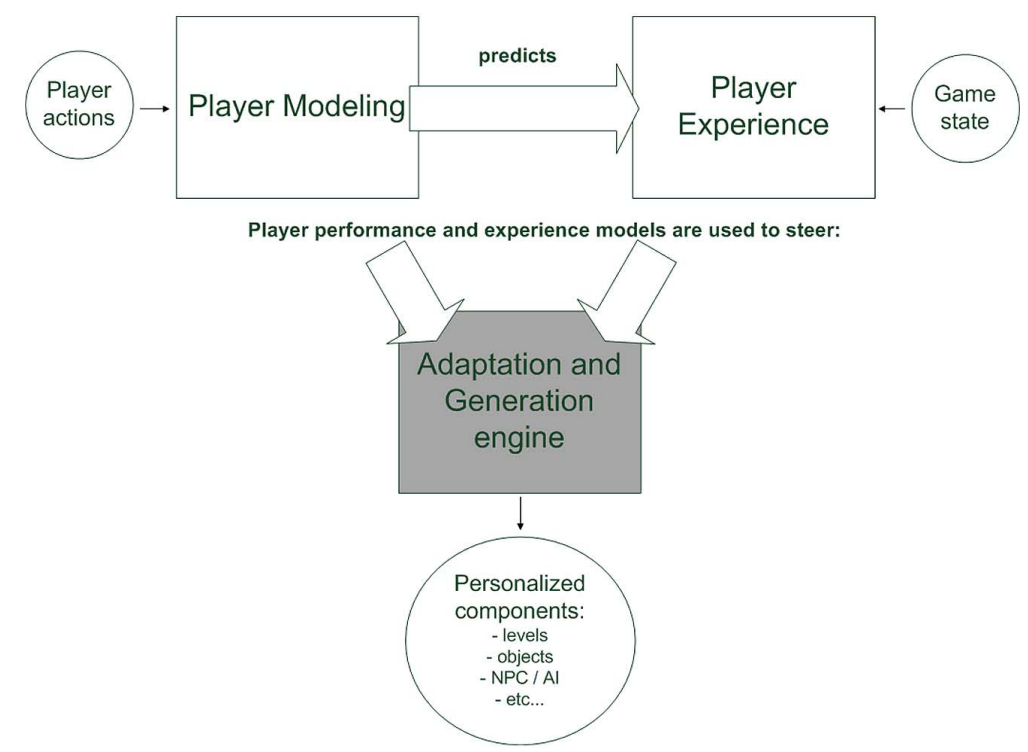
\includegraphics[width=0.75\textwidth]{ch2ddaarch}
	\caption{Přehled principů architektury adaptivních her. \cite{16Survey} }
	\label{fig:ch2ddaarch}
\end{figure}

V \cite{SwPatterns} se zabývali modelem DDA z pohledu návrhových vzorů objektového programování. Abstraktní model je znázorněn na obr. \ref{fig:ch2ddapatterns}. Senzory sbírají důležitá herní data, dle kterých se bude dále rozhodovat. Návrhový vzor Observer je připojen k Senzorům a v případě, že zaznamená zatelnou změnu v systému, vytvoří událost, trigger. Jednotlivé události jsou spojeny s akcemi a dohromady spolu tvoří pravidla uložená v databázi. V případě, že se spustí trigger spojený s akcí v některém z pravidel, rozhodne se v provedení této akce, což má na starost řadič, který má za úkol provést požadovanou změnu do stavu hry.

\begin{figure}
  \centering
  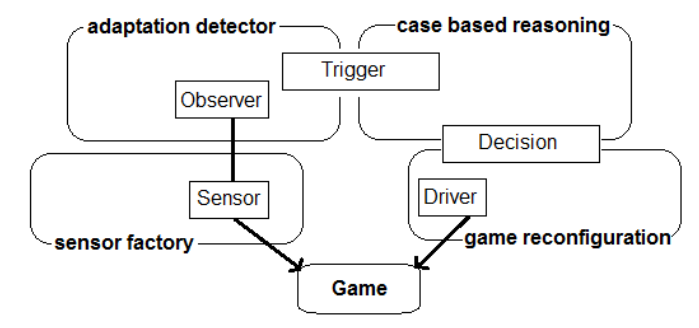
\includegraphics[width=0.75\textwidth]{ch2ddapatterns}
	\caption{Návrhové vzory DDA \cite{SwPatterns} }
	\label{fig:ch2ddapatterns}
\end{figure}

Dále se podíváme na jednotlivé návrhové vzory detailněji.

\subsection{Sensor factory}

Senzory jsou objekty, které pravidelně čtou herní data\footnote{Senzory nemusí zaznamenávat pouze herní data. Mohou zaznamenávat i prostředí uživatele např. pomocí Kinectu, nebo snímat aktuální tep hráče.} a upozorňují na změny zbytek DDA systému. Schéma návrhového vzoru znázorňuje obr. \ref{fig:ch2senzorfactory}. Senzor je abstraktní třídou, která zahrnuje periodické sbírání dat a upozorňující mechanismus. Konkrétní senzory z této třídy dědí a musí přepisovat abstraktní metodu refreshValue(), která zaznamenává konkrétní proměnnou systému. Třída SenzorFactory je zodpovědná za vytváření jednotlivých senzorů a je implementací návrhového vzoru factory. Továrna na senzory vyžaduje název senzoru a objekt, který má monitorovat. Vytvořené senzory si ukládá do registru. V případě, že uživatel zažádá o senzor, který už někdo vytvořil, dostane referenci na tento senzor. V opačném případě zkontroluje v ResourceManageru, jestli vytvořením nového senzoru se poruší některá z omezení zdrojů a pokud ne, senzor vytvoří.

\begin{figure}
  \centering
  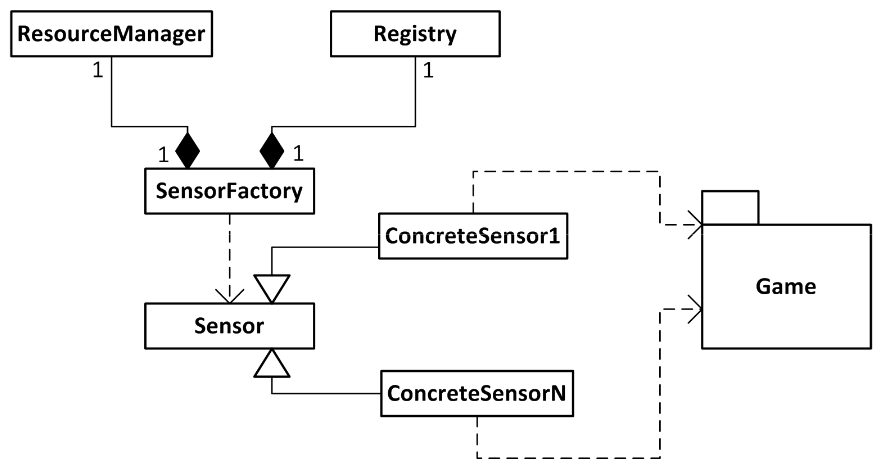
\includegraphics[width=0.5\textwidth]{ch2senzorfactory}
	\caption{Návrhový vzor sensor factory. \cite{SwPatterns} }
	\label{fig:ch2senzorfactory}
\end{figure}

\subsection{Adaptation detector}

Hrubá data získaná senzory se musí dále zpracovat. Tyto data získává AdaptationDetector pomocí observeru z návrhového vzoru senzor-observer. Na tomto místě se rozhoduje, jestli senzory již zaznamenaly dostatečnou změnu systému. Nedostatečnou změnou může být vystřelení jednoho náboje z plně nabitého revolveru. Naopak vystřílení půlky zásobníku může být významné. O významnost změny se stará TreshholdAnalyzer s Tresholdem. Treshold uchovává parametr hranice a její typ. (menší rovno, větší apod.) V případě dosažení prahu TresholdAnalyzer dá vědět AdaptationDetectoru, který vytvoří trigger, spouštěč. Trigger s sebou může nést další dodatečné informace jako je např. množství přeživších nepřátel. Viz obr. \ref{fig:ch2adaptationdesing}.

\begin{figure}
  \centering
  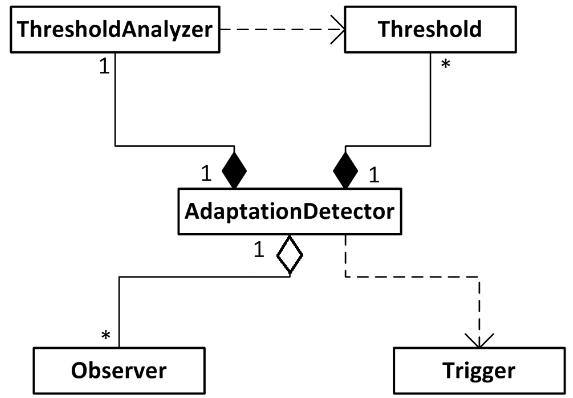
\includegraphics[width=0.5\textwidth]{ch2adaptationdesing}
	\caption{Návrhový vzor sensor factory. \cite{SwPatterns} }
	\label{fig:ch2adaptationdesing}
\end{figure}

\subsection{Case based reasoning}

Trigger spustí rozhodování na základě případů. Tento návrhový vzor(obr. \ref{fig:ch2casebase}) se použije, jestliže je možné vyvažování obtížnosti definovat konečným množstvím případů. InferenceEngine obsahuje dvě datové struktury: TriggerPool a FixedRules. Fixed rules obsahují pravidla, která jsou úzce spojená s konkrétní hrou. Pravidlo je kombinací triggeru a akce/rozhodnutí. TriggerPool funguje jako fronta událostí. Do fronty se řadí spuštěné triggery a jsou obsluhovány od nejstaršího. InferenceEngine vždy odebere jeden trigger z poolu, najde ho v databázi FixedRules pravidel a s ním nalezne vhodné rozhodnutí, které se má dále provést.

\begin{figure}
  \centering
  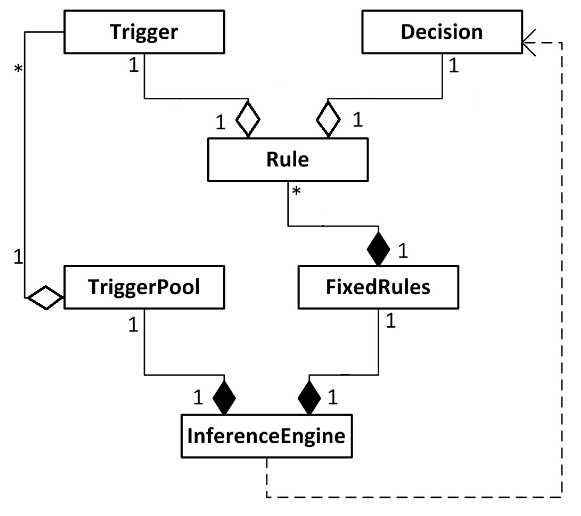
\includegraphics[width=0.5\textwidth]{ch2casebase}
	\caption{Návrhový vzor Case based reasoning. \cite{SwPatterns} }
	\label{fig:ch2casebase}
\end{figure}

\subsection{Game reconfiguration}

Posledním krokem je provedení požadované změny v herním světě. Návrhový vzor Game reconfiguration(obr. \ref{fig:ch2gamereco}) v sobě obsahuje jiný návrhový vzor, adapter. AdaptationDriver dostane ke zpracování rozhodnutí z InferenceEnginu. AdaptationDriver provede rozhodnutí za pomoci Driveru. Driver mění objekty, jež implementují rozhraní State, přes které zjišťuje aktuální stav objektu. S provedením jeho změny čeká dokud se nestane objekt neaktivním.

\begin{figure}
  \centering
  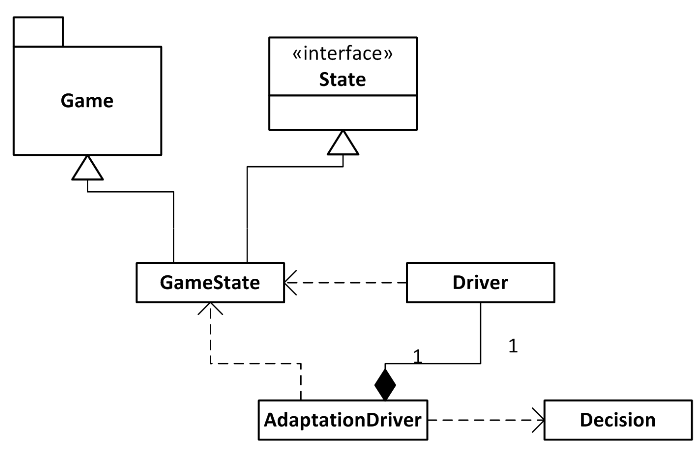
\includegraphics[width=0.5\textwidth]{ch2gamereco}
	\caption{Návrhový vzor Game reconfiguration. \cite{SwPatterns} }
	\label{fig:ch2gamereco}
\end{figure}

\section{Zábava}

Pojem zábava patří mezi velice subjektivní pojmy. Pro každého je zábavného něco jiného a svět her není výjimkou. Mezi hlavní zastupitele zkoumající tento pozitivní požitek patří Mihaly Csikszentmihalyi, který ideální stav maximální zábavy, maximálního ponoření do některé z činností nazval flow. Blíže tento stav bude popsán v následující podsekci.

Přestože se jedná o pojem subjektivní, pro použití DDA je nutné najít některé složky zábavy, které jsou změřitelné, kvantifikovatelné. Musíme být schopni zábavu měřit. Jestliže ji dokážeme změřit, můžeme to využít pro stavbu DDA algoritmů a i pro měření kvalit různých algoritmů mezi sebou. Možné metriky budou popsány dále.

\subsection{Flow}

Flow (tok) je stav mysli, kdy je osoba v průběhu provozování činnosti naprosto soustředěná, pociťuje nadšení, úspěch. „Flow je stav vědomí, kdy je člověk plně zaujatý svou činností. Nezabývá se jinými stimuly z okolí ani svými myšlenkami nebo pocity. Je naprosto soustředěný na prováděnou činnost. Dosahuje většinou, na své poměry, nadprůměrných výkonů, ale přitom mu to nepůsobí výraznou námahu. Je to harmonický zážitek, kdy tělo a mysl spolu bez námahy spolupracují. Tento stav je většinou spojen s pocity energie, radosti, harmonie a seberealizace.“ \cite{FlowCZ} S pojmem Flow prvně přišel zástupce pozitivní psychologie Mihaly Csikszentmihalyi ve své práci Flow: The psychology of optimal experience, česky vydané pod názvem O štěstí a smyslu života.

Požadovaný stav lze charakterizovat z pohledu dovedností člověka a náročnosti prováděné činnosti. Dosáhneme ho, jestliže provádíme úkol náročností odpovídající našim schopnostem. Viz obr. \ref{fig:ch2flow}. 

Jestliže se člověk seznamuje s novou činností, začíná v levém dolním rohu flow grafu. V tu chvíli nemá žádné dovednosti a pravděpodobně se začíná učit provádět činnost od jednoduchých částí po složitější. V knize \cite{OptimalFun} uvádí Csikszentmihalyi jako příklad takové činnosti hraní tenisu a vysvětluje to na obr. \ref{fig:ch2flow}. Alex začíná hrát tenis, a tedy se nachází ve fázi označené $A_1$. Alex v této chvíli neumí vůbec hrát tenis a začíná s tréninkem trefování se do míčku. Není to příliš obtížné, ale Alex si to užívá, protože náročnost tohoto úkolu přesně odpovídá jeho schopnostem.

\begin{figure}
  \centering
  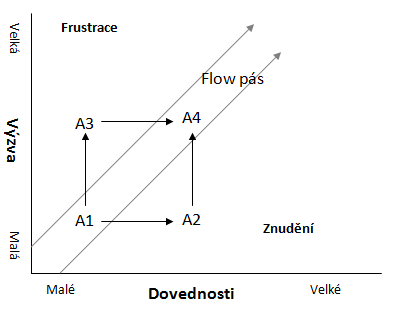
\includegraphics[width=0.5\textwidth]{ch2flow}
	\caption{Příklad pohybu jedince ve flow grafu. \cite{OptimalFun} }
	\label{fig:ch2flow}
\end{figure}

V této chvíli se Alex pohybuje v tzv flow pásu. Na stejném místě v diagramu nemůže zůstat Alex věčně. Jak danou činnost procvičuje, stává se v ní čím dál lepší, přestává ho to bavit, dostává se do nudy znázorněné v grafu $A_2$. V opačném případě se může stát, že potká zkušeného hráče. Hra proti němu je mnohem náročnějším úkolem a převyšuje Alexovy schopnosti. Alex se v takovém případě dostává do stavu úzkosti a stresu $A_3$.

V obou zmíněných příkladech se Alex nachází mimo flow pás a bude se snažit do něj opět dostat. V horším případě hru vzdá a další stav $A_4$ již v grafu nebude. V případě, že je ve stavu $A_2$, je dalším logickým krokem začít obtížnější úkol, vytyčit si nový cíl odpovídající jeho schopnostem. Ve stavu stresu $A_3$ má Alex jedinou možnost, zlepšit své dovednosti, aby se opět vrátil do flow pásu. Teoreticky může ubrat na výzvě, náročnosti úkolu, ale jak je jednou člověk vystaven takové výzvě, je pro něj těžké ji ignorovat a vzdát se jí. \cite{OptimalFun}

Dle Csikszentmihalyi se flow skládá z devíti elementů. \cite{FlowEng} Ne všechny jsou nutně potřebné k dosažení stavu flow.

\begin{enumerate}
	\item Jasné cíle
	\item Zpětná vazba
	\item Vyrovnanost náročnosti úkolů a schopností
	\item Splynutí činnosti a vědomí
	\item Koncentrace
	\item Žádné obavy z neúspěchu
	\item Pocit kontroly
	\item Změna vnímání času
	\item Vnitřní motivace
\end{enumerate}

Rozepisování jednotlivých bodů není záměrem této práce. Bližší informace lze nalézt např. na \cite{FlowEng}, \cite{FlowCZ}, nebo v originální knize \cite{OptimalFun}.

\subsubsection{Flow ve hrách}

Nás bude více zajímat napojení flow na vývoj počítačových her. Jenova Chen ve své diplomové práci Flow in Games\cite{thesisflow} vybral několik flow komponent, které označil za hlavní při návrhu hry. Dle Chena musí hra obsahovat následující tři elementy, aby hráč dosáhl stavu flow.

\begin{enumerate}
	\item Předpokladem je, že hra sama o sobě je pro hráče odměňující. Hráč sám o sobě chce hru hrát.
	\item Hra nabízí správnou náročnost úkolů vzhledem k hráčovým schopnostem, což mu umožňuje více se do hry ponořit.
	\item Hráč potřebuje cítit kontrolu nad prováděnou činností.
\end{enumerate}

Jsou-li splněny všechny tři body, hráč může ztratit pojem o čase a zcela se do hry ponořit.

Stavem flow ve hrách se dále zabýval Lennart Nacket, který ve svém článku\cite{FlowAll} shrnuje spojení flow s počítačovými hrami od různých autorů. Sweetserův a Wyethův herní flow osmi složkami vycházejícími z 9 složek flow od M. Csikszentmihalyi.

\begin{enumerate}
  \item Jasné cíle
	\item Zpětná vazba
	\item Výzva
	\item Hráčovi dovednosti
	\item Koncentrace
	\item Pocit kontroly
	\item Ponoření se do činnosti
	\item Sociální interakce
\end{enumerate}

\textbf{Jasné cíle} : 
Hráč by měl být vždy schopen kognitivně zpracovávat herní mise, úrovně, úkoly. Aktuální úkoly by měly být vždy jednoznačné a nematoucí. Hráč by měl být schopen vnímat svůj pokrok ve hře.

\textbf{Zpětná vazba} : 
Hra by měla vždy uživatele informovat o výsledku provedených akcí. Hráč by měl být seznámen, jak se blíží, či oddaluje od splnění cíle hry.

\textbf{Výzva} : 
U příliš jednoduchých her se nemohou uživatelé ponořit do hry. Hra musí být výzvou. Podstatné je rozlišovat náročnost ve formě špatně navrženého uživatelského rozhraní a ovládání a výzvu jako část herního designu. Špatné ovládání není nikdy žádoucí.

\textbf{Hráčovi dovednosti} : 
Hra by měla být navržena tak, aby hráči umožňovala efektivní získávání herních dovedností. Hra by měla brát v úvahu i možné dovednosti získané hráčem z jiných her.

\textbf{Koncentrace} : 
Hráč musí být do hry zcela ponořen, věnovat ji veškerou svojí pozornost.

\textbf{Pocit kontroly} : 
Hráč má mít pocit, že ovládá dění ve hře. Tento bod může být kritickým u návrhu DDA. Zjistí-li hráč, že jeho úspěch ve hře není zcela závislý na jeho výkonu, ztrácí pocit kontroly.

\textbf{Ponoření se do činnosti} : 
Podobné koncentraci. Hra má pohlcovat a udržovat hráče v maximální pozornosti, ale tak, aby mu to bylo stále příjemné.

\textbf{Sociální interakce} : 
Tento bod je přidán oproti prvotnímu flow. K dokonalému zážitku potřebuje člověk další lidské spoluhráče a protihráče.

\subsubsection{Zóna flow pro různé hráče}

Vraťme se znovu ke flow diagramu \ref{fig:ch2flow}. Dle příkladu s Alexem a jeho učením se tenisu by se mohlo zdát, že pro každého je ideální udržovat zcela vyrovnanou hodnotu schopností a náročnosti úkolů a udržovat uživatele v úzkém flow pásu, jak znázorňuje obr. \ref{fig:ch2flowzone1}.

\begin{figure}
  \centering
  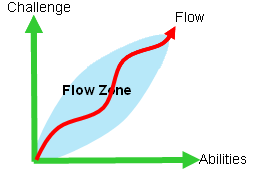
\includegraphics[width=0.5\textwidth]{ch2flowzone1}
	\caption{Obecně je vhodné hráče udržovat ve flow zóně. \cite{thesisflow} }
	\label{fig:ch2flowzone1}
\end{figure}	

Bohužel takový flow diagram nebere v úvahu individualitu hráče. Existují hráči, kteří mají rádi větší výzvy než jsou v tu chvíli schopni zvládnout, lze je nazvat hardcore hráči. Naopak existují příležitostní hráči, kteří netouží po velkých výzvách a nejraději se budou pohybovat lehce pod flow zónou. Těchto specifik si všímá např. práce \cite{RiskTakers}. Ideální průběh hry pro příležitostné/začínající hráče, běžné hráče a hardcore hráče znázorňuje graf na obr. \ref{fig:ch2flowzone2}. Mnohé práce tato specifika opomíjejí a často je jejich cílem upravit obtížnost hry, aby byl vyrovnaný počet hráčových výher a proher a už neberou v potaz, že někteří hráči přestanou hrát, když budou z poloviny pokusů prohrávat.

\begin{figure}
  \centering
  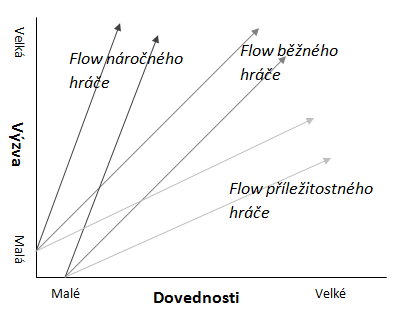
\includegraphics[width=0.5\textwidth]{ch2flowzone2}
	\caption{Flow zóna a specifika pro příležitostné a hardcore hráče. \cite{thesisflow} }
	\label{fig:ch2flowzone2}
\end{figure}	

\subsection{Metriky zábavnosti} \label{sec:defzab}

Hlavním cílem počítačových her je pobavení hráče. Může být tedy dobré umět zábavu přímo, či nepřímo změřit. Pro techniku DDA je existence takové metriky zcela zásadní. Bez ní by hra nevěděla, jakým způsobem se má přizpůsobovat hráči a neuměla by ohodnotit, jestli to dělá dobře. 

Metriky můžeme rozdělit do několika kategorií. Některé metriky jsou specifické pro konkrétní hru, jiné jsou obecně použitelné pro většinu existujících her. Dále jsou metriky, jež vycházejí pouze ze stavu hry, softwaru. Protikladem mohou být speciální metriky měřící hodnoty z vnějšího světa. Příkladem může sledování srdečního tepu \cite{7}. Dále lze využít webkameru, senzory na herních i neherních zařízení. Kromě tepu lze využívat např. pevnost stisku joysticku, měnící se odpor kůže, teplotu těla.\cite{16Survey} V této práci se pro naše účely zaměřím na metriky univerzálně použitelné a získané ze stavu hry.

Zábava ve hrách se často zjednodušuje do podoby náročnosti hry vzhledem k dovednostem hráče. Z tohoto důvodu velké množství přístupů pracuje s metrikami, které zábavu měří nepřímo, měří obtížnost hry. Často používanou metrikou je hodnota win-rate, poměr vítězstvích hráče ku jeho prohrám. Hodnota 0,5 značí polovinu výher a polovinu proher. Mnohé přístupy hodnotu 0,5 berou jako ideální. V tomto případě se hra snaží obtížnosti přiblížit co nejpřesněji dovednostem hráče. Jak bylo naznačeno v předchozí sekci, ne každý hráč ocení polovinu proher. Zde je prostor pro kombinaci statické a dynamické obtížnosti. Při statické obtížnosti si hráč vybere jednu z předem daných obtížností, např. začátečník, pokročilý, expert, kterým budou odpovídat hodnoty win-rate 25, 50, 75 %.

Další metriky využívají heuristiku, která numericky ohodnotí stav hry pro každého hráče a která nepřímo vyjadřuje pravděpodobnost výhry hráče. Samotná heuristika je herně specifická, ale prakticky u každé hry lze nějakou vymyslet, a proto jsou metriky, které ji využívají, obecně použitelné. 

V článku \cite{24DynLev} na základě zmíněné heuristiky přicházejí k třem metrikám. Počet změn ve vedení, napínavost během a konečný výsledek. Hráč, který dle heuristiky má největší pravděpodobnost na výhru je ve vedení. Jestliže se dostane do vedení jiný hráč, zaznamená se to. Metrika měří počet výměn hráčů během hry od začátku do konce. Je zde předpoklad, že hra je více zábavná, jestliže se hráči častěji ve vedení střídají, a tedy není pořadí hráčů stejné na začátku, během a na konci hry. Napínavost hry souvisí s rozptylem heuristiky pro jednotlivé hráče. Hra je napínavější, jestliže všichni hráči mají stejnou pravděpodobnost na výhru během celé hry. První z metrik počítá průměrnou napínavost během hry. Druhá udává o kolik vítěz vyhrál na ostatními hráči.

Všechny 4 zmíněné metriky (3 předchozí + win-rate) lze dobře využít v teorii her pro ohodnocení jednotlivých algoritmů a porovnání jich mezi sebou. Osobně mi počet změn hráčů na chvostu nepřijde jako dostatečný údaj. Mohlo by se stát, že každý z hráčů by byl během hry 2 krát ve vedení, ale jeden z nich by byl ve vedení 90\% času a zbylí hráči zbývajících 10\%. 5. metrika může znázorňovat dobu ve vedení pro každého hráče, nebo rozptyl těchto hodnot jako sjednocující údaj.

Jednou ze složek flow je kontrola. Hráč chce mít pocit vlády nad hrou. Jestliže budeme hru příliš často a hodně přizpůsobovat hráči, on/a si může všimnout, že nemá plnou kontrolu nad hrou, hra ho může přestat bavit. Proto by počet zásahů do hry měl být minimální. Spočítáme si pro každého hráče heuristiku pravděpodobnosti na vítězství vždy před adaptivním krokem $h_1$ a po něm $h_2$. Rozdíl $\Delta h = h_2 - h_1$ znázorňuje, jak moc jsme konkrétnímu hráči ublížili/pomohli k vítězství.  Můžeme vytvořit nové 2 metriky, kontrola a spravedlnost. Kontrola bude dána sumou absolutních hodnot $\Delta h$ během hry. Trochu paradoxně, čím menší hodnota kontroly, tím lépe. Tím méně bylo zasaženo do hry. Pro spravedlnost je důležité během hry pomáhat/ubližovat všem přibližně stejně. Čím vyrovnanější suma $\Delta h$ na konci hry mezi jednotlivými hráči, tím lépe.


  %...

  %\startAppendices
  %  \chapter{Ovládání aplikace}

\section{Aplikace}

Aplikace byla naprogramována v jazyce C++ a používá knihovnu funkcí Qt. Na CD je přiložen projekt pro Visual Studio 2010 se všemi zdrojovými kódy. Dále je k dispozici zkompilovaná verze programu s potřebnými dynamickými knihovnami.

Pro spuštění zkompilované verze je potřeba pouze počítač s operačním systémem Windows. Aplikace se neinstaluje, stačí spuštění .exe souboru.

Ovládání aplikace by mělo být intuitivní. V hlavním menu jsou volby Nová hra, Změnit hru, Nastavení a Dávkové spouštění. Nová hra restartuje hru s novým nastavením. Ve změnit hru lze vybrat jednu ze tří implementovaných her a v Nastavení ji nakonfigurovat.

Menu Dávkové spouštění slouží k provádění experimentů. Zpět z Dávkového spouštění se uživatel dostane vybráním Nová hra z hlavní nabídky.


\begin{figure}
  \centering
  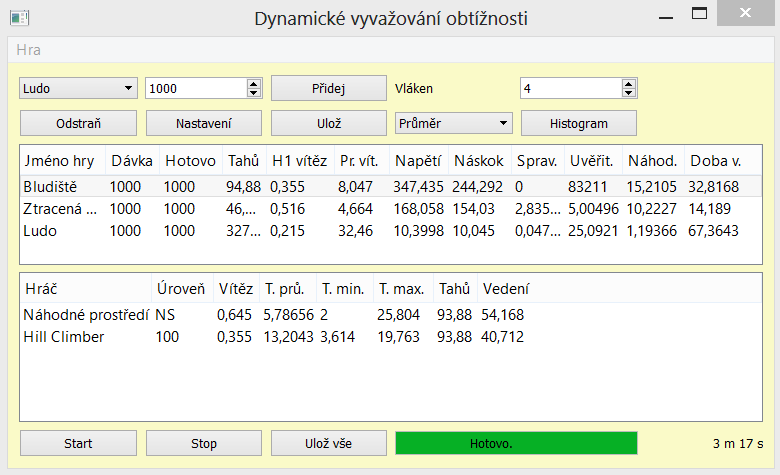
\includegraphics[width=0.90\textwidth]{appdavka}
	\caption{Uživatelské rozhraní dávkového spouštění experimentů. }
	\label{fig-appdavka}
\end{figure}

Uživatel přidá novou dávku zvolením dvou parametrů. Z výběrového menu vybere hru a nastaví počet iterací experimentu. Tlačítkem Přidej vytvoří jeden nový experiment, který se objeví v seznamu navolených experimentů. 

Po označení experimentu v seznamu může uživatel využívat čtveřici tlačítek Odstraň, Nastavení, Ulož, Histogram. Odstraň vymaže experiment z dávky, Nastavení otevře okno s nastavením pro hru, Ulož umožňuje uložit výsledky proběhlého experimentu, Histogram otevře okno, v kterém lze zobrazit jednotlivé metriky pro jeden experiment jako histogram. Dále je ve stejném řádku možnost voleb Průměr, Směrodatná odchylka, Minimum a Maximum. Dle volby se po proběhnutí experimentů v jejich seznamu zobrazují příslušné hodnoty z daných experimentů. 

\begin{figure}
  \centering
  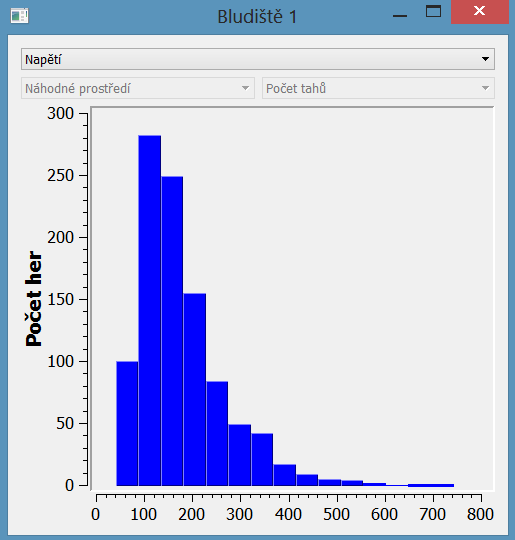
\includegraphics[width=0.75\textwidth]{apphistogram}
	\caption{Histogram metriky Napětí pro hru bludiště a 1000 iterací experimentu. }
	\label{fig-apphistogram}
\end{figure}

Pomocí tlačítka Start se spustí navolené experimenty jeden za druhým. Iterace v rámci jednoho experimentu se rozdělí do předem definovaného počtu vláken. Tlačítkem Stop se experimenty zastaví, ale nechají se doběhnout aktuálně rozehrané hry. Pomocí tlačítka Uložit vše lze hromadně uložit výsledky všech experimentů do zvolené složky. 

V průběhu experimentu se zobrazuje uplynulý čas a velice hrubý odhad skončení experimentů. Spočítá se dle průměrné doby na jednu iteraci od začátku spuštění experimentů a dle počtu zbylých iterací ve všech experimentech.

Po označení experimentu v seznamu se zároveň zobrazí ve spodním okně několik metrik k jednotlivým hráčům. Pro každého hráče je uvedeno jeho jméno, úroveň, poměr vítězství. T. prů. T. min., T. max. značí průměrný, minimální a maximální počet tahů hráče během hry. Poslední dvě metriky znamenají kolikrát byl hráč na tahu a kolik kol byl ve vedení.

V seznamu experimentů se zobrazuje jméno hry, celkový a proběhlý počet iterací experimentu, celkový počet tahů, poměr vítězství prvního hráče a metriky prohození vítězů, napětí, náskok, spravedlnost, uvěřitelnost, náhodnost, doba vedení v tomto pořadí.

\section{Hry}

V této části stručně popíši uživatelské rozhraní jednotlivých her. Nezmiňuji zde pravidla her, která byla uvedena v páté kapitole.

Nastavení her je stejné pro dávkové spouštění i při hraní člověk proti počítači. V levé polovině uživatel může nastavit algoritmy pro jednotlivé hráče a případně jejich úroveň, pokud to daný algoritmus umožňuje. Pod nastavením hráčů jsou speciální nastavení pro jednotlivé hry popsány níže.

V pravé části nastavení se volí hráč prostředí a koeficienty pro jednotlivé metriky. Nastavení se stane platné až po uložení tlačítkem Uložit a po spuštění nové hry.

\subsection{Bludiště}

Hra se ovládá pomocí levého tlačítka myši. Hráč ovládá žlutou kuličku a snaží se dostat včas ke všem bombám, které jsou na mapě znázorněny zelenými čtverci. Hráč vždy kliknutím vybere, které další dveře se mají otevřít. K otevřeným dveřím postava dojde skokem. Dveře jsou znázorněny oranžovými, modrými a červenými čtverci. Dle barvy dveří a jejich vzdálenosti od předchozí pozice, se hráči odečtou zbývající kroky do konce hry.

\begin{figure}
  \centering
  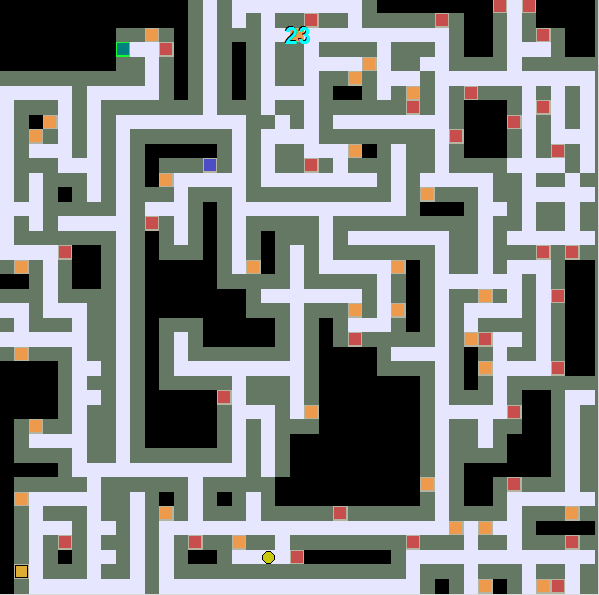
\includegraphics[width=0.75\textwidth]{appmaze}
	\caption{Uživatelské rozhraní hry Bludiště. Zelený čtverec představuje možnou bombu. }
	\label{fig-appmaze}
\end{figure}

Zbývající počet kroků do konce hry zobrazuje tyrkysové číslo v horní části hry. 

V případě, že některá bomba se stane nedostupnou, tak byla falešná a zmizí z mapy.

\emph{Speciální nastavení} : Před hrou hráč může upravit parametry velikosti bludiště a počáteční limit na počet kroků.

\subsection{Ludo}

Hra Ludo se také ovládá pomocí myši. Kostkou se hází automaticky. Hodnota, která padla, je znázorněna uprostřed herní plochy. Hráč může pohnout s figurami, které jsou na bíle zvýrazněném poli. Jestliže figurkou nemůže pohnout, tak buď mu v tom brání vlastní figurka, kterou by jinak vyhodil, nebo je před figurkou již obsazené bezpečné místo.

\begin{figure}
  \centering
  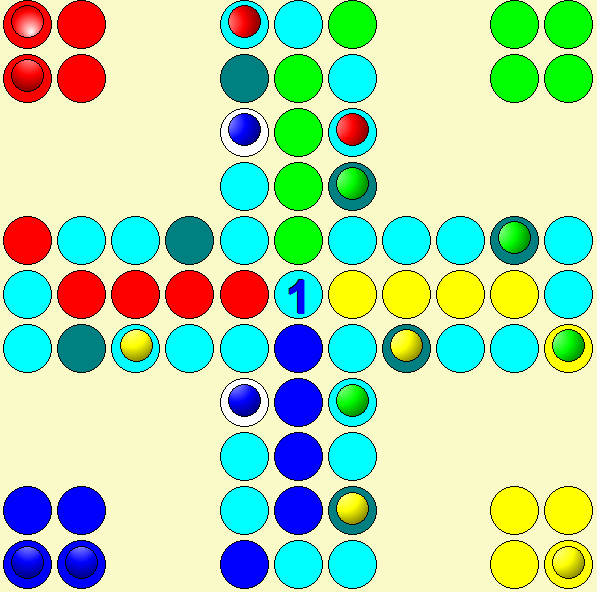
\includegraphics[width=0.75\textwidth]{appludo}
	\caption{Uživatelské rozhraní hry Ludo. Bílý podklad značí aktivní figurky. }
	\label{fig-appludo}
\end{figure}

Bezpečná místa jsou zvýrazněna tmavší barvou.

V případě, že hráč nemá ani jednu figurkou na hlavním plánu, hází kostkou až třikrát. Pouze první hod se provede automaticky, ostatní hody provádí hráč kliknutím doprostřed herního pole.

\emph{Speciální nastavení} : Lze nastavit hru pouze dvou hráčů. V takovém případě se ignoruje nastavení druhého a čtvrtého hráče.

\subsection{Ztracená města}

Hra se opět ovládá pouze pomocí levého tlačítka myši. Každý tah se vždy skládá ze třech kliknutí. Prvním kliknutím na kartu v ruce hráč vybere, s kterou kartou bude hrát. 

Při druhém kliknutí hráč vybírá, co s kartou udělá. Může jí buď zahodit vybráním příslušného odkládacího balíčku, které jsou na začátku hry znázorněny šedivým čtvercem se zaoblenými hranami. V případě, že kartu může zahrát, klikne pod odkládací balíček dané barvy. 


\begin{figure}
  \centering
  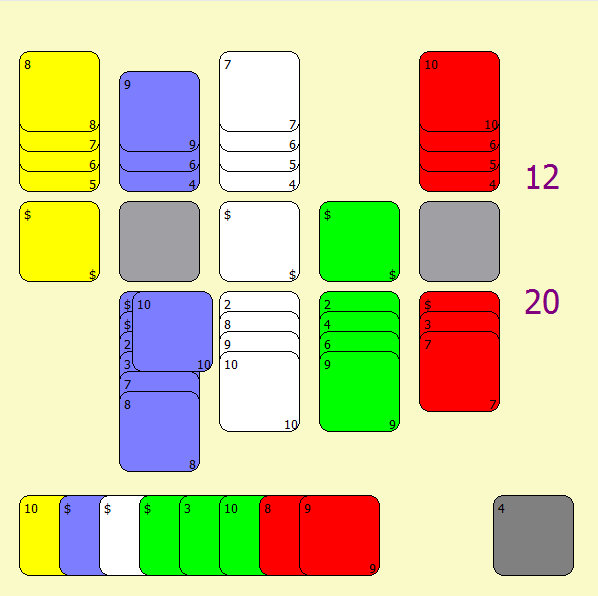
\includegraphics[width=0.75\textwidth]{applc}
	\caption{Uživatelské rozhraní hry Ztracená města. }
	\label{fig-applc}
\end{figure}

Nakonec třetím kliknutím hráč vybere, odkud dobere kartu. Jedna z možností je dobrat z dobíracího balíčku, který je znázorněn šedivě v pravém dolním rohu. Je na něm číslo udávající počet zbývajících karet v balíčku. V případě, že jsou na stole odložené karty, může hráč kliknout na jednu z nich a vzít si ji do ruky.

Uživateli se vždy zvýrazňují oblasti ve hře, které jsou zrovna aktivní a hráč na ně může kliknout.

\emph{Speciální nastavení} : Lze nastavit počet karet v ruce. Oficiální pravidla hry umožňují variantu 8 a 5 karet v ruce.

\endinput
%%
%% End of file `ch01.tex'.

  %\stopAppendices
\stopBodyMatter

\startBackMatter
  \PrintBibliography
  %\PrintIndex % define index entry in the text by: \index{word}
\stopBackMatter

\end{document}

\endinput
%%
%% End of file `template.tex'.
